\documentclass[twoside]{book}

% Packages required by doxygen
\usepackage{fixltx2e}
\usepackage{calc}
\usepackage{doxygen}
\usepackage[export]{adjustbox} % also loads graphicx
\usepackage{graphicx}
\usepackage[utf8]{inputenc}
\usepackage{makeidx}
\usepackage{multicol}
\usepackage{multirow}
\PassOptionsToPackage{warn}{textcomp}
\usepackage{textcomp}
\usepackage[nointegrals]{wasysym}
\usepackage[table]{xcolor}

% Font selection
\usepackage[T1]{fontenc}
\usepackage[scaled=.90]{helvet}
\usepackage{courier}
\usepackage{amssymb}
\usepackage{sectsty}
\renewcommand{\familydefault}{\sfdefault}
\allsectionsfont{%
  \fontseries{bc}\selectfont%
  \color{darkgray}%
}
\renewcommand{\DoxyLabelFont}{%
  \fontseries{bc}\selectfont%
  \color{darkgray}%
}
\newcommand{\+}{\discretionary{\mbox{\scriptsize$\hookleftarrow$}}{}{}}

% Page & text layout
\usepackage{geometry}
\geometry{%
  a4paper,%
  top=2.5cm,%
  bottom=2.5cm,%
  left=2.5cm,%
  right=2.5cm%
}
\tolerance=750
\hfuzz=15pt
\hbadness=750
\setlength{\emergencystretch}{15pt}
\setlength{\parindent}{0cm}
\setlength{\parskip}{3ex plus 2ex minus 2ex}
\makeatletter
\renewcommand{\paragraph}{%
  \@startsection{paragraph}{4}{0ex}{-1.0ex}{1.0ex}{%
    \normalfont\normalsize\bfseries\SS@parafont%
  }%
}
\renewcommand{\subparagraph}{%
  \@startsection{subparagraph}{5}{0ex}{-1.0ex}{1.0ex}{%
    \normalfont\normalsize\bfseries\SS@subparafont%
  }%
}
\makeatother

% Headers & footers
\usepackage{fancyhdr}
\pagestyle{fancyplain}
\fancyhead[LE]{\fancyplain{}{\bfseries\thepage}}
\fancyhead[CE]{\fancyplain{}{}}
\fancyhead[RE]{\fancyplain{}{\bfseries\leftmark}}
\fancyhead[LO]{\fancyplain{}{\bfseries\rightmark}}
\fancyhead[CO]{\fancyplain{}{}}
\fancyhead[RO]{\fancyplain{}{\bfseries\thepage}}
\fancyfoot[LE]{\fancyplain{}{}}
\fancyfoot[CE]{\fancyplain{}{}}
\fancyfoot[RE]{\fancyplain{}{\bfseries\scriptsize Generated by Doxygen }}
\fancyfoot[LO]{\fancyplain{}{\bfseries\scriptsize Generated by Doxygen }}
\fancyfoot[CO]{\fancyplain{}{}}
\fancyfoot[RO]{\fancyplain{}{}}
\renewcommand{\footrulewidth}{0.4pt}
\renewcommand{\chaptermark}[1]{%
  \markboth{#1}{}%
}
\renewcommand{\sectionmark}[1]{%
  \markright{\thesection\ #1}%
}

% Indices & bibliography
\usepackage{natbib}
\usepackage[titles]{tocloft}
\setcounter{tocdepth}{3}
\setcounter{secnumdepth}{5}
\makeindex

% Hyperlinks (required, but should be loaded last)
\usepackage{ifpdf}
\ifpdf
  \usepackage[pdftex,pagebackref=true]{hyperref}
\else
  \usepackage[ps2pdf,pagebackref=true]{hyperref}
\fi
\hypersetup{%
  colorlinks=true,%
  linkcolor=blue,%
  citecolor=blue,%
  unicode%
}

% Custom commands
\newcommand{\clearemptydoublepage}{%
  \newpage{\pagestyle{empty}\cleardoublepage}%
}

\usepackage{caption}
\captionsetup{labelsep=space,justification=centering,font={bf},singlelinecheck=off,skip=4pt,position=top}

%===== C O N T E N T S =====

\begin{document}

% Titlepage & ToC
\hypersetup{pageanchor=false,
             bookmarksnumbered=true,
             pdfencoding=unicode
            }
\pagenumbering{alph}
\begin{titlepage}
\vspace*{7cm}
\begin{center}%
{\Large Genetix \\[1ex]\large 0.\+1 }\\
\vspace*{1cm}
{\large Generated by Doxygen 1.8.13}\\
\end{center}
\end{titlepage}
\clearemptydoublepage
\pagenumbering{roman}
\tableofcontents
\clearemptydoublepage
\pagenumbering{arabic}
\hypersetup{pageanchor=true}

%--- Begin generated contents ---
\chapter{Hierarchical Index}
\section{Class Hierarchy}
This inheritance list is sorted roughly, but not completely, alphabetically\+:\begin{DoxyCompactList}
\item \contentsline{section}{data}{\pageref{structdata}}{}
\item \contentsline{section}{eval}{\pageref{structeval}}{}
\item \contentsline{section}{nodo}{\pageref{structnodo}}{}
\item \contentsline{section}{Player}{\pageref{classPlayer}}{}
\begin{DoxyCompactList}
\item \contentsline{section}{AI}{\pageref{classAI}}{}
\item \contentsline{section}{Random}{\pageref{classRandom}}{}
\item \contentsline{section}{Tester}{\pageref{classTester}}{}
\item \contentsline{section}{Umano}{\pageref{classUmano}}{}
\end{DoxyCompactList}
\item Q\+Object\begin{DoxyCompactList}
\item \contentsline{section}{Brain}{\pageref{classBrain}}{}
\item \contentsline{section}{Client}{\pageref{classClient}}{}
\item \contentsline{section}{Game\+Abstract}{\pageref{classGameAbstract}}{}
\begin{DoxyCompactList}
\item \contentsline{section}{Game}{\pageref{classGame}}{}
\end{DoxyCompactList}
\item \contentsline{section}{Worker}{\pageref{classWorker}}{}
\end{DoxyCompactList}
\item Q\+Tcp\+Server\begin{DoxyCompactList}
\item \contentsline{section}{Distributed\+Network}{\pageref{classDistributedNetwork}}{}
\end{DoxyCompactList}
\item Q\+Thread\begin{DoxyCompactList}
\item \contentsline{section}{Engine}{\pageref{classEngine}}{}
\item \contentsline{section}{Sleeper}{\pageref{classSleeper}}{}
\item \contentsline{section}{T}{\pageref{classT}}{}
\end{DoxyCompactList}
\item Q\+Widget\begin{DoxyCompactList}
\item \contentsline{section}{Client\+Window}{\pageref{classClientWindow}}{}
\item \contentsline{section}{Main\+Window}{\pageref{classMainWindow}}{}
\end{DoxyCompactList}
\item \contentsline{section}{stat}{\pageref{structstat}}{}
\item \contentsline{section}{Style}{\pageref{classStyle}}{}
\item \contentsline{section}{Table}{\pageref{classTable}}{}
\item \contentsline{section}{Tree}{\pageref{classTree}}{}
\end{DoxyCompactList}

\chapter{Class Index}
\section{Class List}
Here are the classes, structs, unions and interfaces with brief descriptions\+:\begin{DoxyCompactList}
\item\contentsline{section}{\hyperlink{classAI}{AI} }{\pageref{classAI}}{}
\item\contentsline{section}{\hyperlink{classBrain}{Brain} }{\pageref{classBrain}}{}
\item\contentsline{section}{\hyperlink{classClient}{Client} }{\pageref{classClient}}{}
\item\contentsline{section}{\hyperlink{classClientWindow}{Client\+Window} }{\pageref{classClientWindow}}{}
\item\contentsline{section}{\hyperlink{structdata}{data} }{\pageref{structdata}}{}
\item\contentsline{section}{\hyperlink{classDistributedNetwork}{Distributed\+Network} \\*The \hyperlink{classDistributedNetwork}{Distributed\+Network} class Gestisce il sistema di calcolo distribuito }{\pageref{classDistributedNetwork}}{}
\item\contentsline{section}{\hyperlink{classEngine}{Engine} }{\pageref{classEngine}}{}
\item\contentsline{section}{\hyperlink{structeval}{eval} }{\pageref{structeval}}{}
\item\contentsline{section}{\hyperlink{classGame}{Game} }{\pageref{classGame}}{}
\item\contentsline{section}{\hyperlink{classGameAbstract}{Game\+Abstract} }{\pageref{classGameAbstract}}{}
\item\contentsline{section}{\hyperlink{classMainWindow}{Main\+Window} }{\pageref{classMainWindow}}{}
\item\contentsline{section}{\hyperlink{structnodo}{nodo} }{\pageref{structnodo}}{}
\item\contentsline{section}{\hyperlink{classPlayer}{Player} \\*Classe astratta che desscrive l\textquotesingle{}interfaccia pubblica di un giocatore }{\pageref{classPlayer}}{}
\item\contentsline{section}{\hyperlink{classRandom}{Random} }{\pageref{classRandom}}{}
\item\contentsline{section}{\hyperlink{classSleeper}{Sleeper} \\*Semplice classe per avere un delay }{\pageref{classSleeper}}{}
\item\contentsline{section}{\hyperlink{structstat}{stat} }{\pageref{structstat}}{}
\item\contentsline{section}{\hyperlink{classStyle}{Style} }{\pageref{classStyle}}{}
\item\contentsline{section}{\hyperlink{classT}{T} }{\pageref{classT}}{}
\item\contentsline{section}{\hyperlink{classTable}{Table} \\*The Tavolo class classe che implementa e gestisce il campo da gioco }{\pageref{classTable}}{}
\item\contentsline{section}{\hyperlink{classTester}{Tester} }{\pageref{classTester}}{}
\item\contentsline{section}{\hyperlink{classTree}{Tree} }{\pageref{classTree}}{}
\item\contentsline{section}{\hyperlink{classUmano}{Umano} }{\pageref{classUmano}}{}
\item\contentsline{section}{\hyperlink{classWorker}{Worker} }{\pageref{classWorker}}{}
\end{DoxyCompactList}

\chapter{Class Documentation}
\hypertarget{classAI}{}\section{AI Class Reference}
\label{classAI}\index{AI@{AI}}


Inheritance diagram for AI\+:
\nopagebreak
\begin{figure}[H]
\begin{center}
\leavevmode
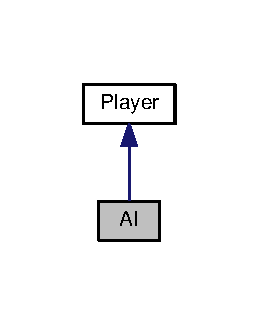
\includegraphics[width=124pt]{classAI__inherit__graph}
\end{center}
\end{figure}


Collaboration diagram for AI\+:
\nopagebreak
\begin{figure}[H]
\begin{center}
\leavevmode
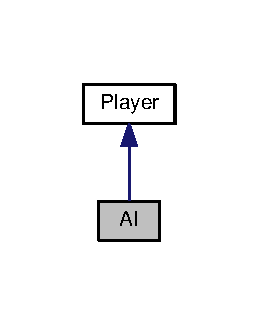
\includegraphics[width=124pt]{classAI__coll__graph}
\end{center}
\end{figure}
\subsection*{Public Member Functions}
\begin{DoxyCompactItemize}
\item 
\mbox{\Hypertarget{classAI_a960e91a972f13b9ee7e9348a2afa6e77}\label{classAI_a960e91a972f13b9ee7e9348a2afa6e77}} 
{\bfseries AI} (\hyperlink{classBrain}{Brain} $\ast$b, int id=-\/1)
\item 
int \hyperlink{classAI_a5ddd05acc3177d4e7a756f7cfc2c3f64}{calcola\+Mossa} (const \hyperlink{classTable}{Table} \&table, int turno) const
\begin{DoxyCompactList}\small\item\em \hyperlink{classAI_a5ddd05acc3177d4e7a756f7cfc2c3f64}{A\+I\+::calcola\+Mossa}. \end{DoxyCompactList}\item 
\mbox{\Hypertarget{classAI_ae83a9db8d9b08b349bc8e089155ab8b4}\label{classAI_ae83a9db8d9b08b349bc8e089155ab8b4}} 
void {\bfseries add\+Score} (float s)
\item 
\mbox{\Hypertarget{classAI_ace2cfc3e36b418f1517965c49941fc82}\label{classAI_ace2cfc3e36b418f1517965c49941fc82}} 
void {\bfseries win} (float s)
\item 
\mbox{\Hypertarget{classAI_a1f9260c8e7d05740078f022fac8e41f7}\label{classAI_a1f9260c8e7d05740078f022fac8e41f7}} 
void {\bfseries lose} (float s)
\item 
\mbox{\Hypertarget{classAI_a2d48915a47b0ba41ab39e7e1d778a861}\label{classAI_a2d48915a47b0ba41ab39e7e1d778a861}} 
void {\bfseries parity} (float s)
\item 
\mbox{\Hypertarget{classAI_a4a2fca8f4558c5eefca6e7a8f72d953f}\label{classAI_a4a2fca8f4558c5eefca6e7a8f72d953f}} 
\hyperlink{structstat}{stat} {\bfseries statistics} () const
\item 
\mbox{\Hypertarget{classAI_ac4c6a612da44dc592114d29daf9a9dea}\label{classAI_ac4c6a612da44dc592114d29daf9a9dea}} 
float {\bfseries get\+Score} () const
\item 
\mbox{\Hypertarget{classAI_aa7e70fc5d035c94be8ee88a928cfb005}\label{classAI_aa7e70fc5d035c94be8ee88a928cfb005}} 
int {\bfseries get\+ID} () const
\item 
\mbox{\Hypertarget{classAI_a5195ab988169b68281a423d3eed1911f}\label{classAI_a5195ab988169b68281a423d3eed1911f}} 
void {\bfseries set\+ID} (int id=-\/1)
\item 
\mbox{\Hypertarget{classAI_a4adef146c29d24ac5a3c5a10f1315834}\label{classAI_a4adef146c29d24ac5a3c5a10f1315834}} 
void {\bfseries reset\+Score} ()
\item 
\mbox{\Hypertarget{classAI_a07c09b5f832f252e117cbdf16e7ae879}\label{classAI_a07c09b5f832f252e117cbdf16e7ae879}} 
bool {\bfseries operator$<$} (const \hyperlink{classPlayer}{Player} \&) const
\end{DoxyCompactItemize}
\subsection*{Static Public Member Functions}
\begin{DoxyCompactItemize}
\item 
\mbox{\Hypertarget{classAI_a864dc398addb033871e745bdd531375b}\label{classAI_a864dc398addb033871e745bdd531375b}} 
static int {\bfseries max\+Value\+Of} (const Q\+Vector$<$ float $>$ v)
\end{DoxyCompactItemize}
\subsection*{Friends}
\begin{DoxyCompactItemize}
\item 
\mbox{\Hypertarget{classAI_a603488eb9c51e35d098875bfef26ae6b}\label{classAI_a603488eb9c51e35d098875bfef26ae6b}} 
\hyperlink{classAI}{AI} $\ast$ {\bfseries operator+} (const \hyperlink{classAI}{AI} \&, const \hyperlink{classAI}{AI} \&)
\item 
\mbox{\Hypertarget{classAI_a4e43a95ad357cdc9a98735958b0c6fa4}\label{classAI_a4e43a95ad357cdc9a98735958b0c6fa4}} 
bool {\bfseries operator$<$} (const \hyperlink{classAI}{AI} \&a, const \hyperlink{classAI}{AI} \&b)
\item 
\mbox{\Hypertarget{classAI_a8685adc9a5fb5397423dd97deef7e733}\label{classAI_a8685adc9a5fb5397423dd97deef7e733}} 
bool {\bfseries operator$<$=} (const \hyperlink{classAI}{AI} \&a, const \hyperlink{classAI}{AI} \&b)
\item 
\mbox{\Hypertarget{classAI_a83c936475bdbb2c3b7a615f26c0b0b20}\label{classAI_a83c936475bdbb2c3b7a615f26c0b0b20}} 
bool {\bfseries operator$>$} (const \hyperlink{classAI}{AI} \&a, const \hyperlink{classAI}{AI} \&b)
\item 
\mbox{\Hypertarget{classAI_a9f2bf11a0a8c5b305e4dfd0bf0b9533d}\label{classAI_a9f2bf11a0a8c5b305e4dfd0bf0b9533d}} 
bool {\bfseries operator$>$=} (const \hyperlink{classAI}{AI} \&a, const \hyperlink{classAI}{AI} \&b)
\end{DoxyCompactItemize}


\subsection{Member Function Documentation}
\mbox{\Hypertarget{classAI_a5ddd05acc3177d4e7a756f7cfc2c3f64}\label{classAI_a5ddd05acc3177d4e7a756f7cfc2c3f64}} 
\index{AI@{AI}!calcola\+Mossa@{calcola\+Mossa}}
\index{calcola\+Mossa@{calcola\+Mossa}!AI@{AI}}
\subsubsection{\texorpdfstring{calcola\+Mossa()}{calcolaMossa()}}
{\footnotesize\ttfamily int A\+I\+::calcola\+Mossa (\begin{DoxyParamCaption}\item[{const \hyperlink{classTable}{Table} \&}]{table,  }\item[{int}]{turno }\end{DoxyParamCaption}) const\hspace{0.3cm}{\ttfamily [virtual]}}



\hyperlink{classAI_a5ddd05acc3177d4e7a756f7cfc2c3f64}{A\+I\+::calcola\+Mossa}. 


\begin{DoxyParams}{Parameters}
{\em tavolo} & \\
\hline
{\em turno} & \\
\hline
\end{DoxyParams}
\begin{DoxyReturn}{Returns}
ritorna la mossa con la valutazione migliore 
\end{DoxyReturn}


Implements \hyperlink{classPlayer}{Player}.



The documentation for this class was generated from the following files\+:\begin{DoxyCompactItemize}
\item 
/home/matteo/\+Progetti/\+Genetix/ai.\+h\item 
/home/matteo/\+Progetti/\+Genetix/ai.\+cpp\end{DoxyCompactItemize}

\hypertarget{classBrain}{}\section{Brain Class Reference}
\label{classBrain}\index{Brain@{Brain}}


Inheritance diagram for Brain\+:
\nopagebreak
\begin{figure}[H]
\begin{center}
\leavevmode
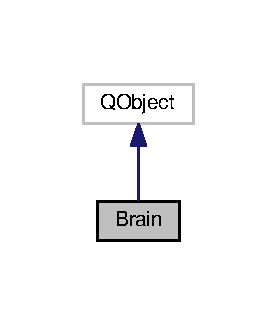
\includegraphics[width=133pt]{classBrain__inherit__graph}
\end{center}
\end{figure}


Collaboration diagram for Brain\+:
\nopagebreak
\begin{figure}[H]
\begin{center}
\leavevmode
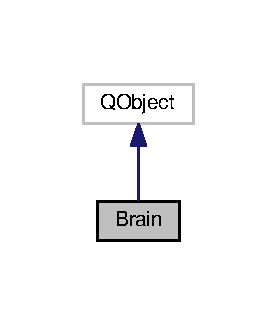
\includegraphics[width=133pt]{classBrain__coll__graph}
\end{center}
\end{figure}
\subsection*{Public Member Functions}
\begin{DoxyCompactItemize}
\item 
\hyperlink{classBrain_ad9637628ba623b059846b435fc11348f}{Brain} (const Q\+Vector$<$ int $>$ \&topology, const Q\+Vector$<$ float $>$ $\ast$weights=0, Q\+Object $\ast$parent=0)
\item 
\mbox{\Hypertarget{classBrain_ab93fdda1e6862ee9c39b443c626747c4}\label{classBrain_ab93fdda1e6862ee9c39b443c626747c4}} 
Q\+Vector$<$ float $>$ {\bfseries get\+Output} (const Q\+Vector$<$ float $>$ \&input)
\item 
\mbox{\Hypertarget{classBrain_aaedc1a6837b5da9e107dd32e4758866c}\label{classBrain_aaedc1a6837b5da9e107dd32e4758866c}} 
void {\bfseries backprop} (const Q\+Vector$<$ float $>$ \&out, const Q\+Vector$<$ float $>$ \&out\+\_\+expct)
\item 
\mbox{\Hypertarget{classBrain_aad7d0a00e9bee1d550a42353ef362327}\label{classBrain_aad7d0a00e9bee1d550a42353ef362327}} 
void {\bfseries print} () const
\item 
\mbox{\Hypertarget{classBrain_afbd471807a2991713cf498d9f8727ac4}\label{classBrain_afbd471807a2991713cf498d9f8727ac4}} 
void {\bfseries info} () const
\item 
\mbox{\Hypertarget{classBrain_af170533115f7495684eeb5926fbcc8cd}\label{classBrain_af170533115f7495684eeb5926fbcc8cd}} 
Q\+Vector$<$ float $>$ \& {\bfseries get\+Weights} ()
\item 
\mbox{\Hypertarget{classBrain_a60c602a02b896c888ceeb357594b9d1e}\label{classBrain_a60c602a02b896c888ceeb357594b9d1e}} 
Q\+Vector$<$ int $>$ \& {\bfseries get\+Topology} ()
\end{DoxyCompactItemize}
\subsection*{Static Public Member Functions}
\begin{DoxyCompactItemize}
\item 
static float \hyperlink{classBrain_acb60a16fa86243d358bb64bfaeee91d0}{rand\+To} (float min, float max)
\begin{DoxyCompactList}\small\item\em \hyperlink{classBrain_acb60a16fa86243d358bb64bfaeee91d0}{Brain\+::rand\+To}. \end{DoxyCompactList}\end{DoxyCompactItemize}
\subsection*{Friends}
\begin{DoxyCompactItemize}
\item 
\mbox{\Hypertarget{classBrain_af6f9db04e9c20020c21c7d1e9750b484}\label{classBrain_af6f9db04e9c20020c21c7d1e9750b484}} 
\hyperlink{classBrain}{Brain} $\ast$ {\bfseries operator+} (const \hyperlink{classBrain}{Brain} \&, const \hyperlink{classBrain}{Brain} \&)
\end{DoxyCompactItemize}


\subsection{Constructor \& Destructor Documentation}
\mbox{\Hypertarget{classBrain_ad9637628ba623b059846b435fc11348f}\label{classBrain_ad9637628ba623b059846b435fc11348f}} 
\index{Brain@{Brain}!Brain@{Brain}}
\index{Brain@{Brain}!Brain@{Brain}}
\subsubsection{\texorpdfstring{Brain()}{Brain()}}
{\footnotesize\ttfamily Brain\+::\+Brain (\begin{DoxyParamCaption}\item[{const Q\+Vector$<$ int $>$ \&}]{topology,  }\item[{const Q\+Vector$<$ float $>$ $\ast$}]{weights = {\ttfamily 0},  }\item[{Q\+Object $\ast$}]{parent = {\ttfamily 0} }\end{DoxyParamCaption})}

calcolo il numero di neuroni e di pesi totali con dei semplici cicli infine ridimensiono ogni vector con la giusta grandezza

\subsection{Member Function Documentation}
\mbox{\Hypertarget{classBrain_acb60a16fa86243d358bb64bfaeee91d0}\label{classBrain_acb60a16fa86243d358bb64bfaeee91d0}} 
\index{Brain@{Brain}!rand\+To@{rand\+To}}
\index{rand\+To@{rand\+To}!Brain@{Brain}}
\subsubsection{\texorpdfstring{rand\+To()}{randTo()}}
{\footnotesize\ttfamily float Brain\+::rand\+To (\begin{DoxyParamCaption}\item[{float}]{min,  }\item[{float}]{max }\end{DoxyParamCaption})\hspace{0.3cm}{\ttfamily [static]}}



\hyperlink{classBrain_acb60a16fa86243d358bb64bfaeee91d0}{Brain\+::rand\+To}. 


\begin{DoxyParams}{Parameters}
{\em max} & \\
\hline
\end{DoxyParams}
\begin{DoxyReturn}{Returns}
float tra min e max 
\end{DoxyReturn}


The documentation for this class was generated from the following files\+:\begin{DoxyCompactItemize}
\item 
/home/matteo/\+Progetti/\+Genetix/brain.\+h\item 
/home/matteo/\+Progetti/\+Genetix/brain.\+cpp\end{DoxyCompactItemize}

\hypertarget{classClient}{}\section{Client Class Reference}
\label{classClient}\index{Client@{Client}}


Inheritance diagram for Client\+:
\nopagebreak
\begin{figure}[H]
\begin{center}
\leavevmode
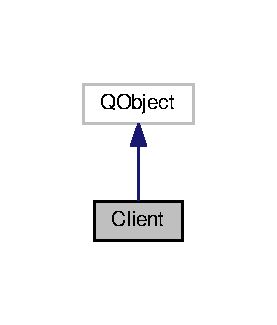
\includegraphics[width=133pt]{classClient__inherit__graph}
\end{center}
\end{figure}


Collaboration diagram for Client\+:
\nopagebreak
\begin{figure}[H]
\begin{center}
\leavevmode
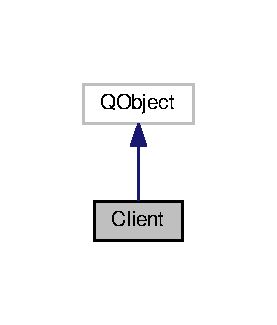
\includegraphics[width=133pt]{classClient__coll__graph}
\end{center}
\end{figure}
\subsection*{Signals}
\begin{DoxyCompactItemize}
\item 
\mbox{\Hypertarget{classClient_a6b2f5f43de87c2d97a6438e467c16b5c}\label{classClient_a6b2f5f43de87c2d97a6438e467c16b5c}} 
void {\bfseries output} (Q\+String)
\item 
\mbox{\Hypertarget{classClient_a5d55e10c7cc67ac9118d43ccce5bec6a}\label{classClient_a5d55e10c7cc67ac9118d43ccce5bec6a}} 
void {\bfseries status} (Q\+Abstract\+Socket\+::\+Socket\+State s)
\end{DoxyCompactItemize}
\subsection*{Public Member Functions}
\begin{DoxyCompactItemize}
\item 
\mbox{\Hypertarget{classClient_a7832757f3fa37f564a21cb2b79b2baad}\label{classClient_a7832757f3fa37f564a21cb2b79b2baad}} 
{\bfseries Client} (Q\+Object $\ast$parent=0)
\item 
\mbox{\Hypertarget{classClient_a7439b9f4cd0a2d745d60c49c2db55935}\label{classClient_a7439b9f4cd0a2d745d60c49c2db55935}} 
void {\bfseries connetti} (Q\+String host=\char`\"{}localhost\char`\"{}, quint16 port=2501)
\end{DoxyCompactItemize}


The documentation for this class was generated from the following files\+:\begin{DoxyCompactItemize}
\item 
/home/matteo/\+Progetti/\+Genetix/client.\+h\item 
/home/matteo/\+Progetti/\+Genetix/client.\+cpp\end{DoxyCompactItemize}

\hypertarget{classClientWindow}{}\section{Client\+Window Class Reference}
\label{classClientWindow}\index{Client\+Window@{Client\+Window}}


Inheritance diagram for Client\+Window\+:
\nopagebreak
\begin{figure}[H]
\begin{center}
\leavevmode
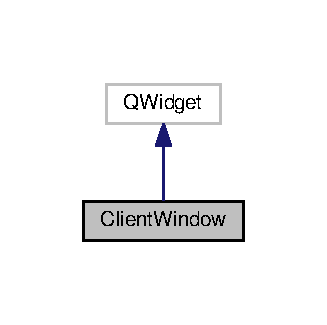
\includegraphics[width=157pt]{classClientWindow__inherit__graph}
\end{center}
\end{figure}


Collaboration diagram for Client\+Window\+:
\nopagebreak
\begin{figure}[H]
\begin{center}
\leavevmode
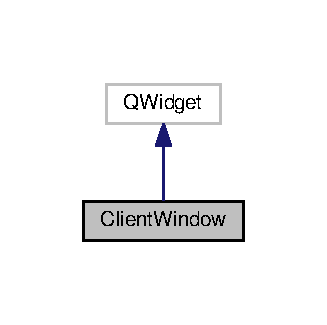
\includegraphics[width=157pt]{classClientWindow__coll__graph}
\end{center}
\end{figure}
\subsection*{Public Slots}
\begin{DoxyCompactItemize}
\item 
\mbox{\Hypertarget{classClientWindow_a8438dfd883dec996752761c7cf3a6218}\label{classClientWindow_a8438dfd883dec996752761c7cf3a6218}} 
void {\bfseries connetti} ()
\item 
\mbox{\Hypertarget{classClientWindow_a3ba1088e8ef18d7203eb848b90fa4460}\label{classClientWindow_a3ba1088e8ef18d7203eb848b90fa4460}} 
void {\bfseries connection\+State} (Q\+Abstract\+Socket\+::\+Socket\+State s)
\end{DoxyCompactItemize}
\subsection*{Public Member Functions}
\begin{DoxyCompactItemize}
\item 
\mbox{\Hypertarget{classClientWindow_a7155f4a6425594dfaf7346575fcf3b40}\label{classClientWindow_a7155f4a6425594dfaf7346575fcf3b40}} 
{\bfseries Client\+Window} (Q\+Widget $\ast$parent=0)
\end{DoxyCompactItemize}


The documentation for this class was generated from the following files\+:\begin{DoxyCompactItemize}
\item 
/home/matteo/\+Progetti/\+Genetix/clientwindow.\+h\item 
/home/matteo/\+Progetti/\+Genetix/clientwindow.\+cpp\end{DoxyCompactItemize}

\hypertarget{structdata}{}\section{data Struct Reference}
\label{structdata}\index{data@{data}}
\subsection*{Public Member Functions}
\begin{DoxyCompactItemize}
\item 
\mbox{\Hypertarget{structdata_ad5a9caebaaee08e701c848b9722e5bf5}\label{structdata_ad5a9caebaaee08e701c848b9722e5bf5}} 
{\bfseries data} (int m, int t)
\end{DoxyCompactItemize}
\subsection*{Public Attributes}
\begin{DoxyCompactItemize}
\item 
\mbox{\Hypertarget{structdata_aa5c1b3aa3b43846e47b1ee08d1d19d3c}\label{structdata_aa5c1b3aa3b43846e47b1ee08d1d19d3c}} 
int {\bfseries mossa}
\item 
\mbox{\Hypertarget{structdata_a893101f17a0ccbc3a40f3661bf95d19e}\label{structdata_a893101f17a0ccbc3a40f3661bf95d19e}} 
int {\bfseries turno}
\end{DoxyCompactItemize}


The documentation for this struct was generated from the following file\+:\begin{DoxyCompactItemize}
\item 
/home/matteo/\+Progetti/\+Genetix/tree.\+h\end{DoxyCompactItemize}

\hypertarget{classDistributedNetwork}{}\section{Distributed\+Network Class Reference}
\label{classDistributedNetwork}\index{Distributed\+Network@{Distributed\+Network}}


The \hyperlink{classDistributedNetwork}{Distributed\+Network} class Gestisce il sistema di calcolo distribuito.  




{\ttfamily \#include $<$distributednetwork.\+h$>$}



Inheritance diagram for Distributed\+Network\+:
\nopagebreak
\begin{figure}[H]
\begin{center}
\leavevmode
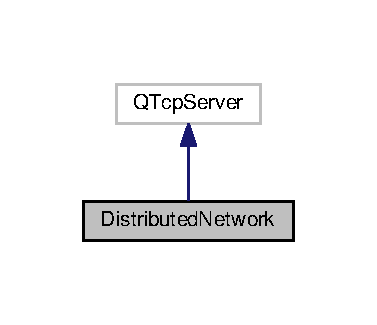
\includegraphics[width=181pt]{classDistributedNetwork__inherit__graph}
\end{center}
\end{figure}


Collaboration diagram for Distributed\+Network\+:
\nopagebreak
\begin{figure}[H]
\begin{center}
\leavevmode
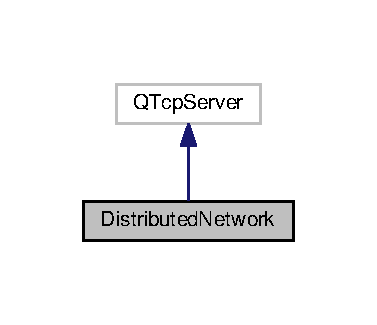
\includegraphics[width=181pt]{classDistributedNetwork__coll__graph}
\end{center}
\end{figure}
\subsection*{Public Slots}
\begin{DoxyCompactItemize}
\item 
\mbox{\Hypertarget{classDistributedNetwork_a55dcd6497ede05e34ead0f59c942d095}\label{classDistributedNetwork_a55dcd6497ede05e34ead0f59c942d095}} 
void {\bfseries new\+Client} ()
\item 
\mbox{\Hypertarget{classDistributedNetwork_a54ee7dae7cbece114adc5c446cbf2e3a}\label{classDistributedNetwork_a54ee7dae7cbece114adc5c446cbf2e3a}} 
void {\bfseries get\+Elab\+Data} (Q\+Byte\+Array \&result)
\item 
\mbox{\Hypertarget{classDistributedNetwork_ab9dc432472463ee387e1b5d40279f8da}\label{classDistributedNetwork_ab9dc432472463ee387e1b5d40279f8da}} 
void {\bfseries client\+Disconnected} (int id, Q\+Byte\+Array \&\hyperlink{structdata}{data})
\end{DoxyCompactItemize}
\subsection*{Signals}
\begin{DoxyCompactItemize}
\item 
\mbox{\Hypertarget{classDistributedNetwork_ac73f8c68da9510d8b1652328cdf0cccf}\label{classDistributedNetwork_ac73f8c68da9510d8b1652328cdf0cccf}} 
void {\bfseries newtask} ()
\item 
\mbox{\Hypertarget{classDistributedNetwork_a162f4648ab9084f44c23d1213884f6d3}\label{classDistributedNetwork_a162f4648ab9084f44c23d1213884f6d3}} 
void {\bfseries send\+Result} (Q\+Byte\+Array \&result)
\end{DoxyCompactItemize}
\subsection*{Public Member Functions}
\begin{DoxyCompactItemize}
\item 
\mbox{\Hypertarget{classDistributedNetwork_a7467bf77e7be95c46e4c7aae6aa3945c}\label{classDistributedNetwork_a7467bf77e7be95c46e4c7aae6aa3945c}} 
{\bfseries Distributed\+Network} (int port=2501, Q\+Object $\ast$parent=0)
\item 
\mbox{\Hypertarget{classDistributedNetwork_ad833b5e8dafeba806b37be3abb5f5821}\label{classDistributedNetwork_ad833b5e8dafeba806b37be3abb5f5821}} 
void {\bfseries start\+Server} (int p)
\item 
\mbox{\Hypertarget{classDistributedNetwork_a339cc5cf3962778664e79cb54c264b18}\label{classDistributedNetwork_a339cc5cf3962778664e79cb54c264b18}} 
void {\bfseries distribute} (Q\+Byte\+Array \hyperlink{structdata}{data})
\item 
\mbox{\Hypertarget{classDistributedNetwork_a7b3220803f522de0dfd1360c1ccde5ba}\label{classDistributedNetwork_a7b3220803f522de0dfd1360c1ccde5ba}} 
void {\bfseries wait} () const
\end{DoxyCompactItemize}


\subsection{Detailed Description}
The \hyperlink{classDistributedNetwork}{Distributed\+Network} class Gestisce il sistema di calcolo distribuito. 

L\+I\+M\+I\+T\+A\+Z\+I\+O\+NI\+: sia questa Classe che la Classe \hyperlink{classClient}{Client} devono essere eseguiti su architetture a 64 bit 

The documentation for this class was generated from the following files\+:\begin{DoxyCompactItemize}
\item 
/home/matteo/\+Progetti/\+Genetix/distributednetwork.\+h\item 
/home/matteo/\+Progetti/\+Genetix/distributednetwork.\+cpp\end{DoxyCompactItemize}

\hypertarget{classEngine}{}\section{Engine Class Reference}
\label{classEngine}\index{Engine@{Engine}}


Inheritance diagram for Engine\+:
\nopagebreak
\begin{figure}[H]
\begin{center}
\leavevmode
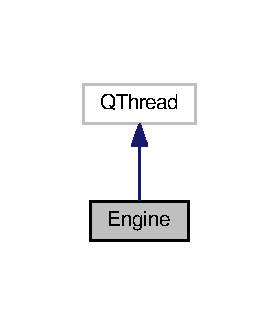
\includegraphics[width=134pt]{classEngine__inherit__graph}
\end{center}
\end{figure}


Collaboration diagram for Engine\+:
\nopagebreak
\begin{figure}[H]
\begin{center}
\leavevmode
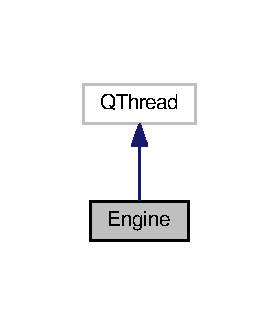
\includegraphics[width=134pt]{classEngine__coll__graph}
\end{center}
\end{figure}
\subsection*{Public Slots}
\begin{DoxyCompactItemize}
\item 
\mbox{\Hypertarget{classEngine_a5b393cd5aaebe5eb8a5b225ee31fa6bb}\label{classEngine_a5b393cd5aaebe5eb8a5b225ee31fa6bb}} 
void {\bfseries run\+Event} ()
\item 
\mbox{\Hypertarget{classEngine_a98956a88f9a0a7e8fedf77cf9c246dd1}\label{classEngine_a98956a88f9a0a7e8fedf77cf9c246dd1}} 
void {\bfseries stop\+Event} ()
\item 
\mbox{\Hypertarget{classEngine_a16bca5737248e72fb0ba519f75adfed0}\label{classEngine_a16bca5737248e72fb0ba519f75adfed0}} 
void {\bfseries set\+Delay} (int)
\item 
\mbox{\Hypertarget{classEngine_ac2275923326b242207830b6a99d37b4a}\label{classEngine_ac2275923326b242207830b6a99d37b4a}} 
void {\bfseries fitness} (Q\+Byte\+Array \&elab)
\end{DoxyCompactItemize}
\subsection*{Signals}
\begin{DoxyCompactItemize}
\item 
\mbox{\Hypertarget{classEngine_a0ce8ae215f05529c846d759f73e3ada9}\label{classEngine_a0ce8ae215f05529c846d759f73e3ada9}} 
void {\bfseries Gen\+Changed} (int new\+Gen)
\item 
\mbox{\Hypertarget{classEngine_a7dfc2258b3a03132a049c8ecfb2d449f}\label{classEngine_a7dfc2258b3a03132a049c8ecfb2d449f}} 
void {\bfseries stop\+Game} ()
\end{DoxyCompactItemize}
\subsection*{Public Member Functions}
\begin{DoxyCompactItemize}
\item 
\mbox{\Hypertarget{classEngine_a8c98683b0a3aa28d8ab72a8bcd0d52f2}\label{classEngine_a8c98683b0a3aa28d8ab72a8bcd0d52f2}} 
\hyperlink{classEngine_a8c98683b0a3aa28d8ab72a8bcd0d52f2}{Engine} ()
\begin{DoxyCompactList}\small\item\em costruttore \end{DoxyCompactList}\item 
\mbox{\Hypertarget{classEngine_ac88ada17b33bc5ddaf6bb73e0cdc67f3}\label{classEngine_ac88ada17b33bc5ddaf6bb73e0cdc67f3}} 
void {\bfseries stop} ()
\item 
\mbox{\Hypertarget{classEngine_a1a210cf30d6bd330b3649439ecd6d6cc}\label{classEngine_a1a210cf30d6bd330b3649439ecd6d6cc}} 
void \hyperlink{classEngine_a1a210cf30d6bd330b3649439ecd6d6cc}{run} ()
\begin{DoxyCompactList}\small\item\em ciclo principale dell\textquotesingle{}algoritmo genetico \end{DoxyCompactList}\item 
int \hyperlink{classEngine_a28dd4d5ff6c82749e651a0254076812a}{save} (Q\+String s=\char`\"{}saves/\char`\"{})
\begin{DoxyCompactList}\small\item\em \hyperlink{classEngine_a28dd4d5ff6c82749e651a0254076812a}{Engine\+::save} funzione che salva lo stato dell\textquotesingle{}\hyperlink{classEngine}{Engine}. \end{DoxyCompactList}\end{DoxyCompactItemize}
\subsection*{Static Public Member Functions}
\begin{DoxyCompactItemize}
\item 
\mbox{\Hypertarget{classEngine_a33c8a56ebe6b872d11f7606035607ce9}\label{classEngine_a33c8a56ebe6b872d11f7606035607ce9}} 
static Q\+Byte\+Array {\bfseries serialize} (Q\+Vector$<$ Player\+Ptr $>$ p)
\item 
\mbox{\Hypertarget{classEngine_aabc5c263d3ec8c61af7656be961af104}\label{classEngine_aabc5c263d3ec8c61af7656be961af104}} 
static Q\+Vector$<$ Player\+Ptr $>$ {\bfseries deserialize} (Q\+Byte\+Array \hyperlink{structdata}{data})
\end{DoxyCompactItemize}


\subsection{Member Function Documentation}
\mbox{\Hypertarget{classEngine_a28dd4d5ff6c82749e651a0254076812a}\label{classEngine_a28dd4d5ff6c82749e651a0254076812a}} 
\index{Engine@{Engine}!save@{save}}
\index{save@{save}!Engine@{Engine}}
\subsubsection{\texorpdfstring{save()}{save()}}
{\footnotesize\ttfamily int Engine\+::save (\begin{DoxyParamCaption}\item[{Q\+String}]{s = {\ttfamily \char`\"{}saves/\char`\"{}} }\end{DoxyParamCaption})}



\hyperlink{classEngine_a28dd4d5ff6c82749e651a0254076812a}{Engine\+::save} funzione che salva lo stato dell\textquotesingle{}\hyperlink{classEngine}{Engine}. 


\begin{DoxyParams}{Parameters}
{\em s} & destinazine del file \\
\hline
\end{DoxyParams}
\begin{DoxyReturn}{Returns}
0 se è andato tutto a buon fine -\/1 se è stato impossibile salvare 
\end{DoxyReturn}


The documentation for this class was generated from the following files\+:\begin{DoxyCompactItemize}
\item 
/home/matteo/\+Progetti/\+Genetix/engine.\+h\item 
/home/matteo/\+Progetti/\+Genetix/engine.\+cpp\end{DoxyCompactItemize}

\hypertarget{structeval}{}\section{eval Struct Reference}
\label{structeval}\index{eval@{eval}}
\subsection*{Public Member Functions}
\begin{DoxyCompactItemize}
\item 
\mbox{\Hypertarget{structeval_a6affabc87a0e79c4678f4c41da7a8550}\label{structeval_a6affabc87a0e79c4678f4c41da7a8550}} 
bool {\bfseries operator$<$} (const \hyperlink{structeval}{eval} \&r) const
\end{DoxyCompactItemize}
\subsection*{Public Attributes}
\begin{DoxyCompactItemize}
\item 
\mbox{\Hypertarget{structeval_a906e05efee4a029df6d3109bf639082f}\label{structeval_a906e05efee4a029df6d3109bf639082f}} 
int {\bfseries mossa}
\item 
\mbox{\Hypertarget{structeval_a992766ff43dde550e1854cc607278560}\label{structeval_a992766ff43dde550e1854cc607278560}} 
float {\bfseries v}
\end{DoxyCompactItemize}


The documentation for this struct was generated from the following file\+:\begin{DoxyCompactItemize}
\item 
/home/matteo/\+Progetti/\+Genetix/ai.\+cpp\end{DoxyCompactItemize}

\hypertarget{classGame}{}\section{Game Class Reference}
\label{classGame}\index{Game@{Game}}


Inheritance diagram for Game\+:
\nopagebreak
\begin{figure}[H]
\begin{center}
\leavevmode
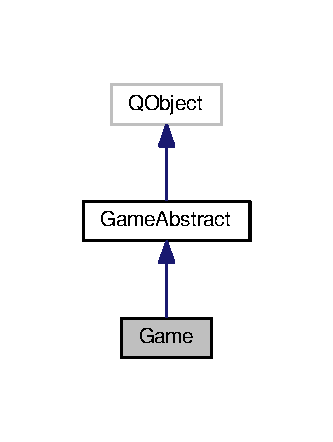
\includegraphics[width=160pt]{classGame__inherit__graph}
\end{center}
\end{figure}


Collaboration diagram for Game\+:
\nopagebreak
\begin{figure}[H]
\begin{center}
\leavevmode
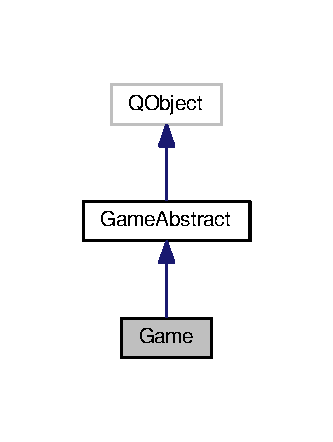
\includegraphics[width=160pt]{classGame__coll__graph}
\end{center}
\end{figure}
\subsection*{Public Slots}
\begin{DoxyCompactItemize}
\item 
\mbox{\Hypertarget{classGame_a17fbb36fd4a2085f9ff4f1fa93d7d08b}\label{classGame_a17fbb36fd4a2085f9ff4f1fa93d7d08b}} 
void {\bfseries stop} ()
\end{DoxyCompactItemize}
\subsection*{Signals}
\begin{DoxyCompactItemize}
\item 
\mbox{\Hypertarget{classGame_a6929ad70cc568687785588a6b5c6d7fc}\label{classGame_a6929ad70cc568687785588a6b5c6d7fc}} 
void {\bfseries output} (Q\+String s)
\end{DoxyCompactItemize}
\subsection*{Public Member Functions}
\begin{DoxyCompactItemize}
\item 
\mbox{\Hypertarget{classGame_a9ea8a3f89f329d2017ef2eec89b58e37}\label{classGame_a9ea8a3f89f329d2017ef2eec89b58e37}} 
{\bfseries Game} (\hyperlink{classEngine}{Engine} $\ast$en=0)
\item 
\mbox{\Hypertarget{classGame_ae31971102f3d122d79d7da1a5672deb5}\label{classGame_ae31971102f3d122d79d7da1a5672deb5}} 
int {\bfseries run} (Q\+Vector$<$ Player\+Ptr $>$ giocatori, \hyperlink{classTree}{Tree} $\ast$tree=nullptr)
\end{DoxyCompactItemize}


The documentation for this class was generated from the following files\+:\begin{DoxyCompactItemize}
\item 
/home/matteo/\+Progetti/\+Genetix/game.\+h\item 
/home/matteo/\+Progetti/\+Genetix/game.\+cpp\end{DoxyCompactItemize}

\hypertarget{classGameAbstract}{}\section{Game\+Abstract Class Reference}
\label{classGameAbstract}\index{Game\+Abstract@{Game\+Abstract}}


Inheritance diagram for Game\+Abstract\+:
\nopagebreak
\begin{figure}[H]
\begin{center}
\leavevmode
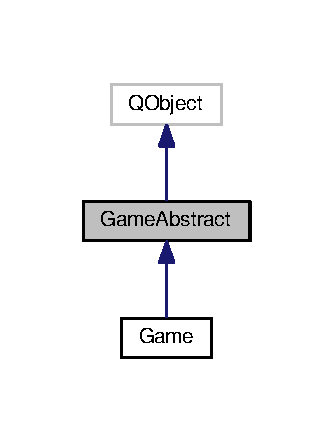
\includegraphics[width=160pt]{classGameAbstract__inherit__graph}
\end{center}
\end{figure}


Collaboration diagram for Game\+Abstract\+:
\nopagebreak
\begin{figure}[H]
\begin{center}
\leavevmode
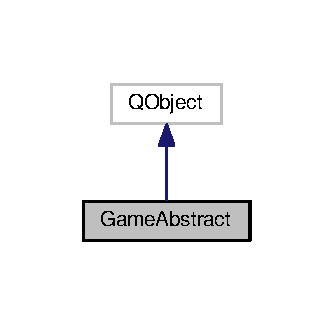
\includegraphics[width=160pt]{classGameAbstract__coll__graph}
\end{center}
\end{figure}
\subsection*{Public Slots}
\begin{DoxyCompactItemize}
\item 
\mbox{\Hypertarget{classGameAbstract_a053f172166edf5e72d80c3266b2b9bfe}\label{classGameAbstract_a053f172166edf5e72d80c3266b2b9bfe}} 
virtual void {\bfseries stop} ()=0
\end{DoxyCompactItemize}
\subsection*{Signals}
\begin{DoxyCompactItemize}
\item 
\mbox{\Hypertarget{classGameAbstract_a00656373d219cc80af1ac277f270da42}\label{classGameAbstract_a00656373d219cc80af1ac277f270da42}} 
virtual void {\bfseries output} (Q\+String s)=0
\end{DoxyCompactItemize}
\subsection*{Public Member Functions}
\begin{DoxyCompactItemize}
\item 
\mbox{\Hypertarget{classGameAbstract_a49ee89bfa47fff6eb177130d0521ab43}\label{classGameAbstract_a49ee89bfa47fff6eb177130d0521ab43}} 
virtual int {\bfseries run} (Q\+Vector$<$ Player\+Ptr $>$ giocatori, \hyperlink{classTree}{Tree} $\ast$)=0
\end{DoxyCompactItemize}


The documentation for this class was generated from the following file\+:\begin{DoxyCompactItemize}
\item 
/home/matteo/\+Progetti/\+Genetix/gameabstract.\+h\end{DoxyCompactItemize}

\hypertarget{classMainWindow}{}\section{Main\+Window Class Reference}
\label{classMainWindow}\index{Main\+Window@{Main\+Window}}


Inheritance diagram for Main\+Window\+:
\nopagebreak
\begin{figure}[H]
\begin{center}
\leavevmode
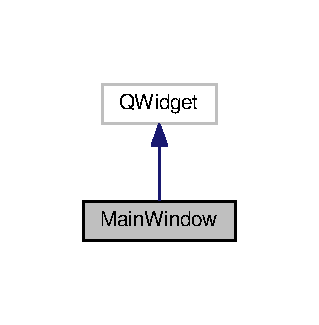
\includegraphics[width=153pt]{classMainWindow__inherit__graph}
\end{center}
\end{figure}


Collaboration diagram for Main\+Window\+:
\nopagebreak
\begin{figure}[H]
\begin{center}
\leavevmode
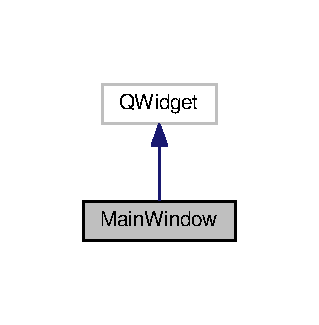
\includegraphics[width=153pt]{classMainWindow__coll__graph}
\end{center}
\end{figure}
\subsection*{Public Slots}
\begin{DoxyCompactItemize}
\item 
\mbox{\Hypertarget{classMainWindow_a7b7807cad6963c4b45483ae68256ea91}\label{classMainWindow_a7b7807cad6963c4b45483ae68256ea91}} 
void {\bfseries changed\+Gen} (int gen)
\item 
\mbox{\Hypertarget{classMainWindow_ae66e9ab15f911b93fce0f161d2fde880}\label{classMainWindow_ae66e9ab15f911b93fce0f161d2fde880}} 
void {\bfseries on\+\_\+start\+\_\+clicked} ()
\item 
\mbox{\Hypertarget{classMainWindow_ac22e784eff724fc28b1c22aa65c4317d}\label{classMainWindow_ac22e784eff724fc28b1c22aa65c4317d}} 
void {\bfseries on\+\_\+stop\+\_\+clicked} ()
\item 
\mbox{\Hypertarget{classMainWindow_a16b98f4e4bc7ff612f2aa7c1eeb70d15}\label{classMainWindow_a16b98f4e4bc7ff612f2aa7c1eeb70d15}} 
void {\bfseries on\+\_\+delay\+\_\+changed} (int)
\end{DoxyCompactItemize}
\subsection*{Signals}
\begin{DoxyCompactItemize}
\item 
\mbox{\Hypertarget{classMainWindow_a4f22c3b06bfbedb52929d213cd5895cb}\label{classMainWindow_a4f22c3b06bfbedb52929d213cd5895cb}} 
void {\bfseries start\+\_\+clicked} ()
\item 
\mbox{\Hypertarget{classMainWindow_a008d7f5813cb95da3885cd60f0e811e5}\label{classMainWindow_a008d7f5813cb95da3885cd60f0e811e5}} 
void {\bfseries stop\+\_\+clicked} ()
\item 
\mbox{\Hypertarget{classMainWindow_aef0d7f0f385563a0805f6dd54c6e90de}\label{classMainWindow_aef0d7f0f385563a0805f6dd54c6e90de}} 
void {\bfseries delay\+\_\+changed} (int)
\end{DoxyCompactItemize}
\subsection*{Public Member Functions}
\begin{DoxyCompactItemize}
\item 
\mbox{\Hypertarget{classMainWindow_a8b244be8b7b7db1b08de2a2acb9409db}\label{classMainWindow_a8b244be8b7b7db1b08de2a2acb9409db}} 
{\bfseries Main\+Window} (Q\+Widget $\ast$parent=0)
\end{DoxyCompactItemize}


The documentation for this class was generated from the following files\+:\begin{DoxyCompactItemize}
\item 
/home/matteo/\+Progetti/\+Genetix/mainwindow.\+h\item 
/home/matteo/\+Progetti/\+Genetix/mainwindow.\+cpp\end{DoxyCompactItemize}

\hypertarget{structnodo}{}\section{nodo Struct Reference}
\label{structnodo}\index{nodo@{nodo}}
\subsection*{Public Member Functions}
\begin{DoxyCompactItemize}
\item 
\mbox{\Hypertarget{structnodo_a9d1dcaed55d5a62573d160779e702911}\label{structnodo_a9d1dcaed55d5a62573d160779e702911}} 
{\bfseries nodo} (int m, int t)
\end{DoxyCompactItemize}
\subsection*{Public Attributes}
\begin{DoxyCompactItemize}
\item 
\mbox{\Hypertarget{structnodo_afe5e9a3e96eac7c82b72117892b83b3d}\label{structnodo_afe5e9a3e96eac7c82b72117892b83b3d}} 
int {\bfseries mossa}
\item 
\mbox{\Hypertarget{structnodo_a69055a314553f4c024db32019bac3e88}\label{structnodo_a69055a314553f4c024db32019bac3e88}} 
int {\bfseries turno}
\item 
\mbox{\Hypertarget{structnodo_af6f1ca1233bca67216c328bc3bbe9a36}\label{structnodo_af6f1ca1233bca67216c328bc3bbe9a36}} 
Q\+Vector$<$ \hyperlink{structnodo}{nodo} $\ast$ $>$ {\bfseries next}
\end{DoxyCompactItemize}


The documentation for this struct was generated from the following file\+:\begin{DoxyCompactItemize}
\item 
/home/matteo/\+Progetti/\+Genetix/tree.\+h\end{DoxyCompactItemize}

\hypertarget{classPlayer}{}\section{Player Class Reference}
\label{classPlayer}\index{Player@{Player}}


classe astratta che desscrive l\textquotesingle{}interfaccia pubblica di un giocatore  




{\ttfamily \#include $<$player.\+h$>$}



Inheritance diagram for Player\+:
\nopagebreak
\begin{figure}[H]
\begin{center}
\leavevmode
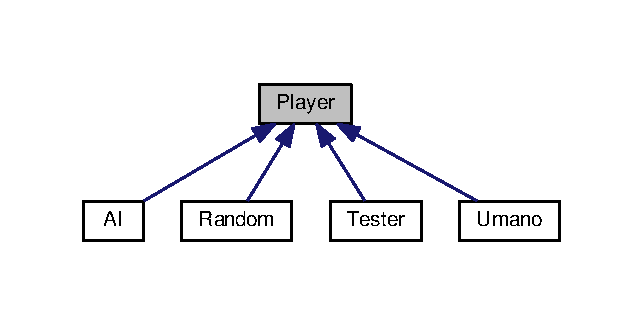
\includegraphics[width=309pt]{classPlayer__inherit__graph}
\end{center}
\end{figure}
\subsection*{Public Member Functions}
\begin{DoxyCompactItemize}
\item 
\mbox{\Hypertarget{classPlayer_a444eb8f2a19debbee8d6dd4a48d846c2}\label{classPlayer_a444eb8f2a19debbee8d6dd4a48d846c2}} 
virtual int {\bfseries calcola\+Mossa} (const \hyperlink{classTable}{Table} \&table, int turno) const =0
\item 
\mbox{\Hypertarget{classPlayer_a776326d11b142ce77092f4ebc8f6e6ad}\label{classPlayer_a776326d11b142ce77092f4ebc8f6e6ad}} 
virtual void {\bfseries add\+Score} (float s)=0
\item 
\mbox{\Hypertarget{classPlayer_aca94f2f4dd3e054c539ecb4c0ac3acda}\label{classPlayer_aca94f2f4dd3e054c539ecb4c0ac3acda}} 
virtual bool {\bfseries operator$<$} (const \hyperlink{classPlayer}{Player} \&) const =0
\item 
\mbox{\Hypertarget{classPlayer_a9c5101d60d359563262426240fdd31c0}\label{classPlayer_a9c5101d60d359563262426240fdd31c0}} 
virtual float {\bfseries get\+Score} () const =0
\item 
\mbox{\Hypertarget{classPlayer_ab8cde15b9f6f3a8c32f310e0ea3e3ae3}\label{classPlayer_ab8cde15b9f6f3a8c32f310e0ea3e3ae3}} 
virtual int {\bfseries get\+ID} () const =0
\item 
\mbox{\Hypertarget{classPlayer_a8a055205512ac51a6bf1b3159000ac7f}\label{classPlayer_a8a055205512ac51a6bf1b3159000ac7f}} 
virtual void {\bfseries set\+ID} (int=-\/1)=0
\item 
\mbox{\Hypertarget{classPlayer_a3bef660a18e4a1366235235b342394ef}\label{classPlayer_a3bef660a18e4a1366235235b342394ef}} 
virtual void {\bfseries reset\+Score} ()=0
\item 
\mbox{\Hypertarget{classPlayer_aad827fcb0d6d140f5188aae38dd95c59}\label{classPlayer_aad827fcb0d6d140f5188aae38dd95c59}} 
virtual void {\bfseries win} (float s)=0
\item 
\mbox{\Hypertarget{classPlayer_a0a3d28e44143a56af896aaa426f9bd30}\label{classPlayer_a0a3d28e44143a56af896aaa426f9bd30}} 
virtual void {\bfseries lose} (float s)=0
\item 
\mbox{\Hypertarget{classPlayer_a2f3a54c4f93737823789b6072a5dfc45}\label{classPlayer_a2f3a54c4f93737823789b6072a5dfc45}} 
virtual void {\bfseries parity} (float s)=0
\item 
\mbox{\Hypertarget{classPlayer_a455902b4c74ae9e63cc86d941bbd2f76}\label{classPlayer_a455902b4c74ae9e63cc86d941bbd2f76}} 
virtual \hyperlink{structstat}{stat} {\bfseries statistics} () const =0
\end{DoxyCompactItemize}


\subsection{Detailed Description}
classe astratta che desscrive l\textquotesingle{}interfaccia pubblica di un giocatore 

The documentation for this class was generated from the following file\+:\begin{DoxyCompactItemize}
\item 
/home/matteo/\+Progetti/\+Genetix/player.\+h\end{DoxyCompactItemize}

\hypertarget{classRandom}{}\section{Random Class Reference}
\label{classRandom}\index{Random@{Random}}


Inheritance diagram for Random\+:
\nopagebreak
\begin{figure}[H]
\begin{center}
\leavevmode
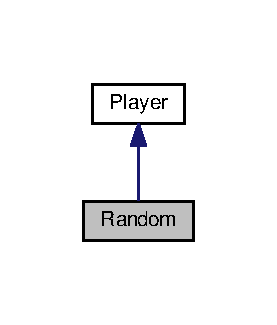
\includegraphics[width=133pt]{classRandom__inherit__graph}
\end{center}
\end{figure}


Collaboration diagram for Random\+:
\nopagebreak
\begin{figure}[H]
\begin{center}
\leavevmode
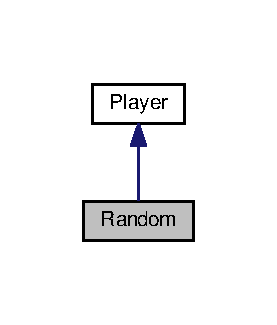
\includegraphics[width=133pt]{classRandom__coll__graph}
\end{center}
\end{figure}
\subsection*{Public Member Functions}
\begin{DoxyCompactItemize}
\item 
\mbox{\Hypertarget{classRandom_a08be0305ca661953e40b4241086d71d2}\label{classRandom_a08be0305ca661953e40b4241086d71d2}} 
int {\bfseries calcola\+Mossa} (const \hyperlink{classTable}{Table} \&table, int turno) const
\item 
\mbox{\Hypertarget{classRandom_a0fa90d0e74f9a26548a7311334ccfe1b}\label{classRandom_a0fa90d0e74f9a26548a7311334ccfe1b}} 
void {\bfseries add\+Score} (float s)
\item 
\mbox{\Hypertarget{classRandom_a154a94c6270445ab9decf58b92f27833}\label{classRandom_a154a94c6270445ab9decf58b92f27833}} 
bool {\bfseries operator$<$} (const \hyperlink{classPlayer}{Player} \&b) const
\item 
\mbox{\Hypertarget{classRandom_a6a114baebd8123b96ae2e65d7d8968e1}\label{classRandom_a6a114baebd8123b96ae2e65d7d8968e1}} 
float {\bfseries get\+Score} () const
\item 
\mbox{\Hypertarget{classRandom_ae06770f8ebf06a18e720fa3ee543d8c2}\label{classRandom_ae06770f8ebf06a18e720fa3ee543d8c2}} 
void {\bfseries reset\+Score} ()
\item 
\mbox{\Hypertarget{classRandom_a2acc914a0a05b81d7d5667c32904e2a3}\label{classRandom_a2acc914a0a05b81d7d5667c32904e2a3}} 
void {\bfseries win} (float s)
\item 
\mbox{\Hypertarget{classRandom_a7e4d72b3d70ea87c89a6ecb073e1d476}\label{classRandom_a7e4d72b3d70ea87c89a6ecb073e1d476}} 
void {\bfseries lose} (float s)
\item 
\mbox{\Hypertarget{classRandom_a9c1b5497aed0a505a1bc9e107b557db4}\label{classRandom_a9c1b5497aed0a505a1bc9e107b557db4}} 
void {\bfseries parity} (float s)
\item 
\mbox{\Hypertarget{classRandom_a5b70e69373f7fd7fb1f20d37edf51b13}\label{classRandom_a5b70e69373f7fd7fb1f20d37edf51b13}} 
\hyperlink{structstat}{stat} {\bfseries statistics} ()
\end{DoxyCompactItemize}


The documentation for this class was generated from the following files\+:\begin{DoxyCompactItemize}
\item 
/home/matteo/\+Progetti/\+Genetix/random.\+h\item 
/home/matteo/\+Progetti/\+Genetix/random.\+cpp\end{DoxyCompactItemize}

\hypertarget{classSleeper}{}\section{Sleeper Class Reference}
\label{classSleeper}\index{Sleeper@{Sleeper}}


semplice classe per avere un delay  




{\ttfamily \#include $<$sleeper.\+h$>$}



Inheritance diagram for Sleeper\+:
\nopagebreak
\begin{figure}[H]
\begin{center}
\leavevmode
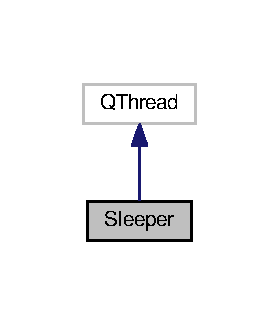
\includegraphics[width=134pt]{classSleeper__inherit__graph}
\end{center}
\end{figure}


Collaboration diagram for Sleeper\+:
\nopagebreak
\begin{figure}[H]
\begin{center}
\leavevmode
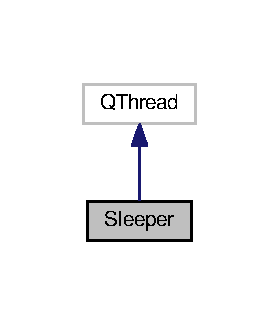
\includegraphics[width=134pt]{classSleeper__coll__graph}
\end{center}
\end{figure}
\subsection*{Static Public Member Functions}
\begin{DoxyCompactItemize}
\item 
\mbox{\Hypertarget{classSleeper_a2990dba95c89499a1164c670159de374}\label{classSleeper_a2990dba95c89499a1164c670159de374}} 
static void {\bfseries usleep} (unsigned long usecs)
\item 
\mbox{\Hypertarget{classSleeper_a88b12fac40c3963b87ac092799dea043}\label{classSleeper_a88b12fac40c3963b87ac092799dea043}} 
static void {\bfseries msleep} (unsigned long msecs)
\item 
\mbox{\Hypertarget{classSleeper_a78d9fd4dfe374ec524960ab32af727b6}\label{classSleeper_a78d9fd4dfe374ec524960ab32af727b6}} 
static void {\bfseries sleep} (unsigned long secs)
\end{DoxyCompactItemize}


\subsection{Detailed Description}
semplice classe per avere un delay 

The documentation for this class was generated from the following files\+:\begin{DoxyCompactItemize}
\item 
/home/matteo/\+Progetti/\+Genetix/sleeper.\+h\item 
/home/matteo/\+Progetti/\+Genetix/sleeper.\+cpp\end{DoxyCompactItemize}

\hypertarget{structstat}{}\section{stat Struct Reference}
\label{structstat}\index{stat@{stat}}
\subsection*{Public Member Functions}
\begin{DoxyCompactItemize}
\item 
\mbox{\Hypertarget{structstat_aacab74c8ceaf07e2e3ff93749dbce025}\label{structstat_aacab74c8ceaf07e2e3ff93749dbce025}} 
{\bfseries stat} (Q\+Vector$<$ int $>$ $\ast$top=0, Q\+Vector$<$ float $>$ $\ast$strat=0, int id=0, float s=0, int w=0, int l=0, int p=0)
\end{DoxyCompactItemize}
\subsection*{Public Attributes}
\begin{DoxyCompactItemize}
\item 
\mbox{\Hypertarget{structstat_ad04ac91884b5e3b802051a36ee1f8c85}\label{structstat_ad04ac91884b5e3b802051a36ee1f8c85}} 
int {\bfseries ID}
\item 
\mbox{\Hypertarget{structstat_a3fa56d7d826bb45c44f259fe54c1fe60}\label{structstat_a3fa56d7d826bb45c44f259fe54c1fe60}} 
float {\bfseries score}
\item 
\mbox{\Hypertarget{structstat_a2ed87c6eae9f14eb89db1e7d3402eb46}\label{structstat_a2ed87c6eae9f14eb89db1e7d3402eb46}} 
int {\bfseries win}
\item 
\mbox{\Hypertarget{structstat_aa7b9c04671338f5e16b45c5b2b6cb874}\label{structstat_aa7b9c04671338f5e16b45c5b2b6cb874}} 
int {\bfseries lose}
\item 
\mbox{\Hypertarget{structstat_affeb64b8e583775f458ade337dfabeae}\label{structstat_affeb64b8e583775f458ade337dfabeae}} 
int {\bfseries parity}
\item 
\mbox{\Hypertarget{structstat_a4a10d6ec8c00498b6ae396f72325655a}\label{structstat_a4a10d6ec8c00498b6ae396f72325655a}} 
Q\+Vector$<$ int $>$ {\bfseries topology}
\item 
\mbox{\Hypertarget{structstat_ad4584c6b45b65ebf4cadf24ea8d9e776}\label{structstat_ad4584c6b45b65ebf4cadf24ea8d9e776}} 
Q\+Vector$<$ float $>$ {\bfseries strategy}
\end{DoxyCompactItemize}
\subsection*{Friends}
\begin{DoxyCompactItemize}
\item 
\mbox{\Hypertarget{structstat_a22be91ddd7908fc418e37946b0faeb6a}\label{structstat_a22be91ddd7908fc418e37946b0faeb6a}} 
std\+::ostream \& {\bfseries operator$<$$<$} (std\+::ostream \&out, const \hyperlink{structstat}{stat} \&s)
\end{DoxyCompactItemize}


The documentation for this struct was generated from the following file\+:\begin{DoxyCompactItemize}
\item 
/home/matteo/\+Progetti/\+Genetix/player.\+h\end{DoxyCompactItemize}

\hypertarget{classStyle}{}\section{Style Class Reference}
\label{classStyle}\index{Style@{Style}}
\subsection*{Static Public Member Functions}
\begin{DoxyCompactItemize}
\item 
\mbox{\Hypertarget{classStyle_a85df87bedbd5eefbad8fb2114f471def}\label{classStyle_a85df87bedbd5eefbad8fb2114f471def}} 
static const char $\ast$$\ast$ {\bfseries logo} ()
\end{DoxyCompactItemize}


The documentation for this class was generated from the following files\+:\begin{DoxyCompactItemize}
\item 
/home/matteo/\+Progetti/\+Genetix/style.\+h\item 
/home/matteo/\+Progetti/\+Genetix/style.\+cpp\end{DoxyCompactItemize}

\hypertarget{classT}{}\section{T Class Reference}
\label{classT}\index{T@{T}}


Inheritance diagram for T\+:
\nopagebreak
\begin{figure}[H]
\begin{center}
\leavevmode
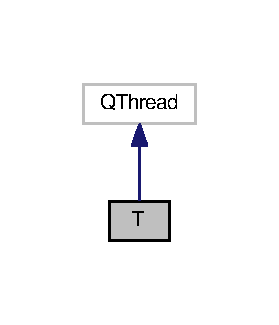
\includegraphics[width=134pt]{classT__inherit__graph}
\end{center}
\end{figure}


Collaboration diagram for T\+:
\nopagebreak
\begin{figure}[H]
\begin{center}
\leavevmode
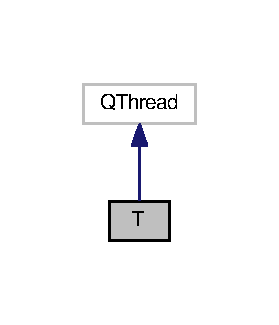
\includegraphics[width=134pt]{classT__coll__graph}
\end{center}
\end{figure}


The documentation for this class was generated from the following file\+:\begin{DoxyCompactItemize}
\item 
/home/matteo/\+Progetti/\+Genetix/main.\+cpp\end{DoxyCompactItemize}

\hypertarget{classTable}{}\section{Table Class Reference}
\label{classTable}\index{Table@{Table}}


The Tavolo class classe che implementa e gestisce il campo da gioco.  




{\ttfamily \#include $<$table.\+h$>$}

\subsection*{Public Member Functions}
\begin{DoxyCompactItemize}
\item 
\mbox{\Hypertarget{classTable_a78948abdf53e4f85773d3e6fabf017d3}\label{classTable_a78948abdf53e4f85773d3e6fabf017d3}} 
void {\bfseries stampa} () const
\item 
\mbox{\Hypertarget{classTable_aeafea436918eac5d5f8968e4cb3d58ca}\label{classTable_aeafea436918eac5d5f8968e4cb3d58ca}} 
Q\+Vector$<$ Q\+Vector$<$ int $>$ $>$ {\bfseries get} () const
\item 
bool \hyperlink{classTable_aa8597647b9049a5403941e3b05cd17cd}{fine\+Gioco} () const
\item 
int \hyperlink{classTable_a23f82e4f0607cb45c4fd834649ad2001}{calcola\+Vincitore} () const
\begin{DoxyCompactList}\small\item\em Tavolo\+::vincitore trova il giocatore che ha vinto la partita. \end{DoxyCompactList}\item 
Q\+Vector$<$ int $>$ \hyperlink{classTable_aa8f05fc3ad41761c70e62e118af5b515}{mosse\+Valide} (int turno) const
\begin{DoxyCompactList}\small\item\em Tavolo\+::mosse\+Valide. \end{DoxyCompactList}\item 
\mbox{\Hypertarget{classTable_aae569e3c7b8606fbbfb7ffcbb0a71607}\label{classTable_aae569e3c7b8606fbbfb7ffcbb0a71607}} 
Q\+Vector$<$ int $>$ {\bfseries mosse\+Non\+Valide} (int turno) const
\item 
int \hyperlink{classTable_ab011fd41be469dd6f67943a596bab4b0}{esegui\+Mossa} (int turno, int mossa)
\begin{DoxyCompactList}\small\item\em Partita\+::controllo. \end{DoxyCompactList}\item 
int \hyperlink{classTable_a6aa69eac7c388df315d1fc7af532cf38}{buche\+Vuote} (int turno) const
\begin{DoxyCompactList}\small\item\em \hyperlink{classTable_a6aa69eac7c388df315d1fc7af532cf38}{Table\+::buche\+Vuote}. \end{DoxyCompactList}\item 
int \hyperlink{classTable_ade5ddf4ac9938a74db6b0d5bb8e9e29a}{differenza\+Punti} (int turno) const
\begin{DoxyCompactList}\small\item\em \hyperlink{classTable_ade5ddf4ac9938a74db6b0d5bb8e9e29a}{Table\+::differenza\+Punti}. \end{DoxyCompactList}\item 
\mbox{\Hypertarget{classTable_a66bac686e8ada4c2617619deb5e06264}\label{classTable_a66bac686e8ada4c2617619deb5e06264}} 
void {\bfseries inizializza} ()
\end{DoxyCompactItemize}
\subsection*{Static Public Member Functions}
\begin{DoxyCompactItemize}
\item 
\mbox{\Hypertarget{classTable_a5bcd33ee120923fa85241da5ede3bc1f}\label{classTable_a5bcd33ee120923fa85241da5ede3bc1f}} 
static int {\bfseries rival} (int turno)
\end{DoxyCompactItemize}


\subsection{Detailed Description}
The Tavolo class classe che implementa e gestisce il campo da gioco. 

\subsection{Member Function Documentation}
\mbox{\Hypertarget{classTable_a6aa69eac7c388df315d1fc7af532cf38}\label{classTable_a6aa69eac7c388df315d1fc7af532cf38}} 
\index{Table@{Table}!buche\+Vuote@{buche\+Vuote}}
\index{buche\+Vuote@{buche\+Vuote}!Table@{Table}}
\subsubsection{\texorpdfstring{buche\+Vuote()}{bucheVuote()}}
{\footnotesize\ttfamily int Table\+::buche\+Vuote (\begin{DoxyParamCaption}\item[{int}]{turno }\end{DoxyParamCaption}) const}



\hyperlink{classTable_a6aa69eac7c388df315d1fc7af532cf38}{Table\+::buche\+Vuote}. 


\begin{DoxyParams}{Parameters}
{\em turno} & \\
\hline
\end{DoxyParams}
\begin{DoxyReturn}{Returns}
numero di buche vuote per il giocatore di turno 
\end{DoxyReturn}
\mbox{\Hypertarget{classTable_a23f82e4f0607cb45c4fd834649ad2001}\label{classTable_a23f82e4f0607cb45c4fd834649ad2001}} 
\index{Table@{Table}!calcola\+Vincitore@{calcola\+Vincitore}}
\index{calcola\+Vincitore@{calcola\+Vincitore}!Table@{Table}}
\subsubsection{\texorpdfstring{calcola\+Vincitore()}{calcolaVincitore()}}
{\footnotesize\ttfamily int Table\+::calcola\+Vincitore (\begin{DoxyParamCaption}{ }\end{DoxyParamCaption}) const}



Tavolo\+::vincitore trova il giocatore che ha vinto la partita. 

\begin{DoxyReturn}{Returns}
0 se ha vinto giocatore 0 1 se ha vinto giocatore 1 2 se pareggio 
\end{DoxyReturn}
\mbox{\Hypertarget{classTable_ade5ddf4ac9938a74db6b0d5bb8e9e29a}\label{classTable_ade5ddf4ac9938a74db6b0d5bb8e9e29a}} 
\index{Table@{Table}!differenza\+Punti@{differenza\+Punti}}
\index{differenza\+Punti@{differenza\+Punti}!Table@{Table}}
\subsubsection{\texorpdfstring{differenza\+Punti()}{differenzaPunti()}}
{\footnotesize\ttfamily int Table\+::differenza\+Punti (\begin{DoxyParamCaption}\item[{int}]{turno }\end{DoxyParamCaption}) const}



\hyperlink{classTable_ade5ddf4ac9938a74db6b0d5bb8e9e29a}{Table\+::differenza\+Punti}. 


\begin{DoxyParams}{Parameters}
{\em turno} & \\
\hline
\end{DoxyParams}
\begin{DoxyReturn}{Returns}
ritorna la differenza punti tra i giocatori $<$ 0 se il giocatore di turno è in svantaggio = 0 se è in parità \begin{quote}
0 se è in vantaggio\end{quote}

\end{DoxyReturn}
\mbox{\Hypertarget{classTable_ab011fd41be469dd6f67943a596bab4b0}\label{classTable_ab011fd41be469dd6f67943a596bab4b0}} 
\index{Table@{Table}!esegui\+Mossa@{esegui\+Mossa}}
\index{esegui\+Mossa@{esegui\+Mossa}!Table@{Table}}
\subsubsection{\texorpdfstring{esegui\+Mossa()}{eseguiMossa()}}
{\footnotesize\ttfamily int Table\+::esegui\+Mossa (\begin{DoxyParamCaption}\item[{int}]{turno,  }\item[{int}]{mossa }\end{DoxyParamCaption})}



Partita\+::controllo. 


\begin{DoxyParams}{Parameters}
{\em turno} & \\
\hline
{\em mossa} & \\
\hline
\end{DoxyParams}
\begin{DoxyReturn}{Returns}
-\/1 se mossa non valida, 0 se fine turno, 1 se ha un altro turno 
\end{DoxyReturn}
\mbox{\Hypertarget{classTable_aa8597647b9049a5403941e3b05cd17cd}\label{classTable_aa8597647b9049a5403941e3b05cd17cd}} 
\index{Table@{Table}!fine\+Gioco@{fine\+Gioco}}
\index{fine\+Gioco@{fine\+Gioco}!Table@{Table}}
\subsubsection{\texorpdfstring{fine\+Gioco()}{fineGioco()}}
{\footnotesize\ttfamily bool Table\+::fine\+Gioco (\begin{DoxyParamCaption}{ }\end{DoxyParamCaption}) const}

if the array of playr 0 or player 1 is all empty then the game is finish

return true if endgame is reached return false if game can be continued \mbox{\Hypertarget{classTable_aa8f05fc3ad41761c70e62e118af5b515}\label{classTable_aa8f05fc3ad41761c70e62e118af5b515}} 
\index{Table@{Table}!mosse\+Valide@{mosse\+Valide}}
\index{mosse\+Valide@{mosse\+Valide}!Table@{Table}}
\subsubsection{\texorpdfstring{mosse\+Valide()}{mosseValide()}}
{\footnotesize\ttfamily Q\+Vector$<$ int $>$ Table\+::mosse\+Valide (\begin{DoxyParamCaption}\item[{int}]{turno }\end{DoxyParamCaption}) const}



Tavolo\+::mosse\+Valide. 


\begin{DoxyParams}{Parameters}
{\em turno} & \\
\hline
\end{DoxyParams}
\begin{DoxyReturn}{Returns}
vettore contenente le mosse possibili per il giocatore di turno 
\end{DoxyReturn}


The documentation for this class was generated from the following files\+:\begin{DoxyCompactItemize}
\item 
/home/matteo/\+Progetti/\+Genetix/table.\+h\item 
/home/matteo/\+Progetti/\+Genetix/table.\+cpp\end{DoxyCompactItemize}

\hypertarget{classTester}{}\section{Tester Class Reference}
\label{classTester}\index{Tester@{Tester}}


Inheritance diagram for Tester\+:
\nopagebreak
\begin{figure}[H]
\begin{center}
\leavevmode
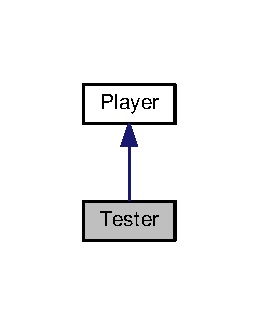
\includegraphics[width=124pt]{classTester__inherit__graph}
\end{center}
\end{figure}


Collaboration diagram for Tester\+:
\nopagebreak
\begin{figure}[H]
\begin{center}
\leavevmode
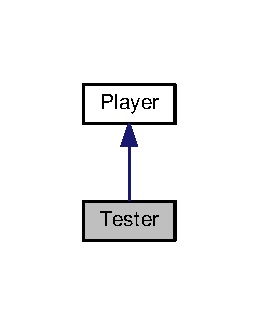
\includegraphics[width=124pt]{classTester__coll__graph}
\end{center}
\end{figure}
\subsection*{Public Member Functions}
\begin{DoxyCompactItemize}
\item 
\mbox{\Hypertarget{classTester_ac7ccbb8c1f95afbcd662688081166ce0}\label{classTester_ac7ccbb8c1f95afbcd662688081166ce0}} 
int {\bfseries calcola\+Mossa} (const \hyperlink{classTable}{Table} \&table, int turno) const
\item 
\mbox{\Hypertarget{classTester_a771e1a605ae0dcf7d1a201b7cb1e9afb}\label{classTester_a771e1a605ae0dcf7d1a201b7cb1e9afb}} 
void {\bfseries add\+Score} (float s)
\item 
\mbox{\Hypertarget{classTester_a166f47c5c14af7202306e7092e76dabb}\label{classTester_a166f47c5c14af7202306e7092e76dabb}} 
bool {\bfseries operator$<$} (const \hyperlink{classPlayer}{Player} \&) const
\item 
\mbox{\Hypertarget{classTester_a535185d2f64e214bea45ee84d193745c}\label{classTester_a535185d2f64e214bea45ee84d193745c}} 
float {\bfseries get\+Score} () const
\item 
\mbox{\Hypertarget{classTester_a330d84c8496c809ed8a3218afbca0431}\label{classTester_a330d84c8496c809ed8a3218afbca0431}} 
void {\bfseries reset\+Score} ()
\item 
\mbox{\Hypertarget{classTester_a36f76c397767071c62a7fe21f7818613}\label{classTester_a36f76c397767071c62a7fe21f7818613}} 
void {\bfseries win} (float s)
\item 
\mbox{\Hypertarget{classTester_a96a762993c9781ccd6817edc6ee30907}\label{classTester_a96a762993c9781ccd6817edc6ee30907}} 
void {\bfseries lose} (float s)
\item 
\mbox{\Hypertarget{classTester_a8292709ff6d1daf1a7998e09892be659}\label{classTester_a8292709ff6d1daf1a7998e09892be659}} 
void {\bfseries parity} (float s)
\item 
\mbox{\Hypertarget{classTester_a0cb4798fcc36d5ce1e0b8a85a6b5c74d}\label{classTester_a0cb4798fcc36d5ce1e0b8a85a6b5c74d}} 
\hyperlink{structstat}{stat} {\bfseries statistics} ()
\end{DoxyCompactItemize}


The documentation for this class was generated from the following files\+:\begin{DoxyCompactItemize}
\item 
/home/matteo/\+Progetti/\+Genetix/tester.\+h\item 
/home/matteo/\+Progetti/\+Genetix/tester.\+cpp\end{DoxyCompactItemize}

\hypertarget{classTree}{}\section{Tree Class Reference}
\label{classTree}\index{Tree@{Tree}}
\subsection*{Public Member Functions}
\begin{DoxyCompactItemize}
\item 
\mbox{\Hypertarget{classTree_aa1849ce447f706f9a3e733c67513eeb6}\label{classTree_aa1849ce447f706f9a3e733c67513eeb6}} 
Q\+Vector$<$ \hyperlink{structdata}{data} $\ast$ $>$ $\ast$ {\bfseries open\+\_\+game} () const
\item 
\mbox{\Hypertarget{classTree_a16bca1b8913f904c4ca7f2cdcb219e89}\label{classTree_a16bca1b8913f904c4ca7f2cdcb219e89}} 
void {\bfseries add} (Q\+Vector$<$ \hyperlink{structdata}{data} $\ast$$>$ \&id)
\item 
\mbox{\Hypertarget{classTree_acaeebec45f26c71162940ddb8664cce2}\label{classTree_acaeebec45f26c71162940ddb8664cce2}} 
void {\bfseries stampa} () const
\item 
\mbox{\Hypertarget{classTree_a203bc7efa4b5a803e306ace63c19384f}\label{classTree_a203bc7efa4b5a803e306ace63c19384f}} 
void {\bfseries info} () const
\end{DoxyCompactItemize}
\subsection*{Public Attributes}
\begin{DoxyCompactItemize}
\item 
\mbox{\Hypertarget{classTree_ae817b42499ec155414dfeb3d6dcda749}\label{classTree_ae817b42499ec155414dfeb3d6dcda749}} 
Q\+Vector$<$ \hyperlink{structnodo}{nodo} $\ast$ $>$ {\bfseries tree}
\end{DoxyCompactItemize}


The documentation for this class was generated from the following files\+:\begin{DoxyCompactItemize}
\item 
/home/matteo/\+Progetti/\+Genetix/tree.\+h\item 
/home/matteo/\+Progetti/\+Genetix/tree.\+cpp\end{DoxyCompactItemize}

\hypertarget{classUmano}{}\section{Umano Class Reference}
\label{classUmano}\index{Umano@{Umano}}


Inheritance diagram for Umano\+:
\nopagebreak
\begin{figure}[H]
\begin{center}
\leavevmode
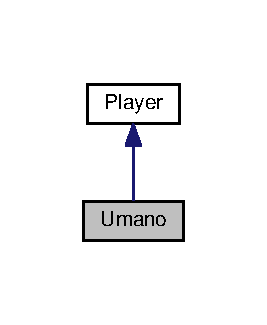
\includegraphics[width=128pt]{classUmano__inherit__graph}
\end{center}
\end{figure}


Collaboration diagram for Umano\+:
\nopagebreak
\begin{figure}[H]
\begin{center}
\leavevmode
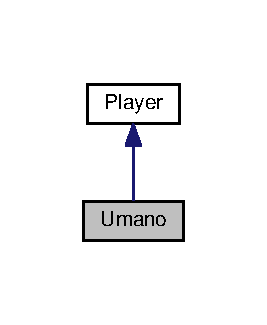
\includegraphics[width=128pt]{classUmano__coll__graph}
\end{center}
\end{figure}
\subsection*{Public Member Functions}
\begin{DoxyCompactItemize}
\item 
\mbox{\Hypertarget{classUmano_aae2b7d9ba681fcda479ae0c7a058f9cf}\label{classUmano_aae2b7d9ba681fcda479ae0c7a058f9cf}} 
int {\bfseries calcola\+Mossa} (const \hyperlink{classTable}{Table} \&table, int turno) const
\item 
\mbox{\Hypertarget{classUmano_a09c8effb9149f8415c594add2a0916d8}\label{classUmano_a09c8effb9149f8415c594add2a0916d8}} 
void {\bfseries add\+Score} (float s)
\item 
\mbox{\Hypertarget{classUmano_a1e3f2122b2d85c4c094500df599be6cc}\label{classUmano_a1e3f2122b2d85c4c094500df599be6cc}} 
float {\bfseries get\+Score} () const
\item 
\mbox{\Hypertarget{classUmano_a5c8477b656066e4b9665e6bb4c61baa4}\label{classUmano_a5c8477b656066e4b9665e6bb4c61baa4}} 
void {\bfseries reset\+Score} ()
\item 
\mbox{\Hypertarget{classUmano_aeab5410ca7202aef8aae1385d6dd4348}\label{classUmano_aeab5410ca7202aef8aae1385d6dd4348}} 
bool {\bfseries operator$<$} (const \hyperlink{classPlayer}{Player} \&) const
\item 
\mbox{\Hypertarget{classUmano_aa1d6cfc4bcbf0db3e2f44a6c4141a02b}\label{classUmano_aa1d6cfc4bcbf0db3e2f44a6c4141a02b}} 
void {\bfseries win} (float s)
\item 
\mbox{\Hypertarget{classUmano_af4f030bea9879a7bc3bbaf1f8ff37f99}\label{classUmano_af4f030bea9879a7bc3bbaf1f8ff37f99}} 
void {\bfseries lose} (float s)
\item 
\mbox{\Hypertarget{classUmano_a18d02c3473b5cfeac64d1dedfb6eb08f}\label{classUmano_a18d02c3473b5cfeac64d1dedfb6eb08f}} 
void {\bfseries parity} (float s)
\item 
\mbox{\Hypertarget{classUmano_a021c553059535dfd141388d689dc4a9c}\label{classUmano_a021c553059535dfd141388d689dc4a9c}} 
\hyperlink{structstat}{stat} {\bfseries statistics} ()
\end{DoxyCompactItemize}


The documentation for this class was generated from the following files\+:\begin{DoxyCompactItemize}
\item 
/home/matteo/\+Progetti/\+Genetix/umano.\+h\item 
/home/matteo/\+Progetti/\+Genetix/umano.\+cpp\end{DoxyCompactItemize}

\hypertarget{classWorker}{}\section{Worker Class Reference}
\label{classWorker}\index{Worker@{Worker}}


Inheritance diagram for Worker\+:
\nopagebreak
\begin{figure}[H]
\begin{center}
\leavevmode
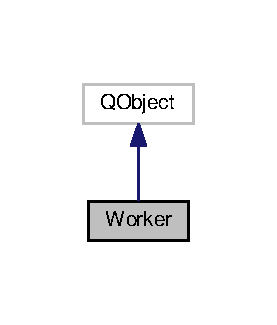
\includegraphics[width=133pt]{classWorker__inherit__graph}
\end{center}
\end{figure}


Collaboration diagram for Worker\+:
\nopagebreak
\begin{figure}[H]
\begin{center}
\leavevmode
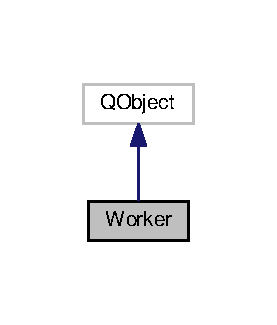
\includegraphics[width=133pt]{classWorker__coll__graph}
\end{center}
\end{figure}
\subsection*{Public Slots}
\begin{DoxyCompactItemize}
\item 
\mbox{\Hypertarget{classWorker_acc404e567293928e2af696bf2ea70999}\label{classWorker_acc404e567293928e2af696bf2ea70999}} 
void {\bfseries read\+Client} ()
\item 
\mbox{\Hypertarget{classWorker_a0917b71f0412691dcab437af6fedb8e6}\label{classWorker_a0917b71f0412691dcab437af6fedb8e6}} 
void {\bfseries get\+Task} ()
\item 
\mbox{\Hypertarget{classWorker_a7c7a418a001835a9ac760b20bd0037ae}\label{classWorker_a7c7a418a001835a9ac760b20bd0037ae}} 
void {\bfseries disconnected} ()
\end{DoxyCompactItemize}
\subsection*{Signals}
\begin{DoxyCompactItemize}
\item 
\mbox{\Hypertarget{classWorker_a1227c92cf569cf361a7a69f13a2e3e1b}\label{classWorker_a1227c92cf569cf361a7a69f13a2e3e1b}} 
void {\bfseries task\+Complete} (Q\+Byte\+Array \&result)
\item 
\mbox{\Hypertarget{classWorker_a94421023a53a3c39d2913ba64980571d}\label{classWorker_a94421023a53a3c39d2913ba64980571d}} 
void {\bfseries disconnected} (int id, Q\+Byte\+Array \&\hyperlink{structdata}{data})
\end{DoxyCompactItemize}
\subsection*{Public Member Functions}
\begin{DoxyCompactItemize}
\item 
\mbox{\Hypertarget{classWorker_af1f07301bce34c5253ac2c2a86945154}\label{classWorker_af1f07301bce34c5253ac2c2a86945154}} 
{\bfseries Worker} (Q\+Tcp\+Socket $\ast$socket, Q\+Queue$<$ Q\+Byte\+Array $>$ \&t, Q\+Mutex \&m)
\item 
\mbox{\Hypertarget{classWorker_a0e11ac035f24a638ab7251f3a3961ac1}\label{classWorker_a0e11ac035f24a638ab7251f3a3961ac1}} 
int {\bfseries get\+ID} ()
\item 
\mbox{\Hypertarget{classWorker_aea9ff3ae949ac3a55ceb51999605887a}\label{classWorker_aea9ff3ae949ac3a55ceb51999605887a}} 
bool {\bfseries is\+Working} ()
\end{DoxyCompactItemize}


The documentation for this class was generated from the following files\+:\begin{DoxyCompactItemize}
\item 
/home/matteo/\+Progetti/\+Genetix/worker.\+h\item 
/home/matteo/\+Progetti/\+Genetix/worker.\+cpp\end{DoxyCompactItemize}

%--- End generated contents ---

% Index
\backmatter
\newpage
\phantomsection
\clearemptydoublepage
\addcontentsline{toc}{chapter}{Index}
\printindex

\end{document}
